\documentclass[a4paper]{article}

\usepackage{INTERSPEECH2021}
\usepackage{adjustbox}
\usepackage{minted}
\usepackage{graphicx}
\usepackage{caption}
\usepackage{subcaption}
\usepackage{graphicx}
\usepackage{tabularray}
\usepackage[dvipsnames]{xcolor}
\definecolor{Mypurple}{HTML}{cc66bd}
\definecolor{Myviolet}{HTML}{8266cc}
\definecolor{Myblue}{HTML}{1f77b4}
\definecolor{Myorange}{HTML}{ff983d}
%\usepackage[showframe]{geometry}% http://ctan.org/pkg/geometry
%\usepackage{lipsum}% http://ctan.org/pkg/lipsum
\newcommand*{\addheight}[2][.5ex]{%
	\raisebox{0pt}[\dimexpr\height+(#1)\relax]{#2}%
}


\title{Final NLU project}
\name{Michele Yin (229359)}

\address{University of Trento}
\email{michele.yin@studenti.unitn.it}

\begin{document}

\maketitle


\section{Introduction}
    Here are presented two neural network based models on the joint task of slot filling and intent classification. The dataset tested are ATIS and SNIPS.
    
    The first model is based on a bidirectional LSTM. 
    The second model consists of fine tuning a pretrained BERT model as backbone.
    Both models use random loss weighting and focal loss to get slightly better results.
    
    Although both are an improvement with respect to a simple baseline model, neither is able to achieve results close to the current state of the art on ATIS and SNIPS for joint slot filling and intent classification. 
        
    
\section{Task Formalisation}
The task consists of two separate, but related tasks, \emph{Slot filling} and \emph{Intent classification}:
\begin{itemize}

\item{\emph{Slot filling}}
defined as: 
\begin{itemize}
	\item given a sequence of tokens $w = {w_1, w_2, ..., w_n}$
	\item defined a sequence of labels as $l = {l_1, l_2, ..., l_n}$
	\item compute the sequence $\hat{l}$ such as $\hat{l} = \underset{l}{\operatorname{argmax}}\text{ }P(l|w)$ 
\end{itemize}


An example from SNIPS dataset is the following: 

\begin{table}[h!]
	\centering
	\begin{adjustbox}{max width=0.5\textwidth}
		\begin{tabular}{*{4}{l}}%%{|c|c|c|c|c|c|c|c|c|c|c|c|c|c|}
%			\hline
%			Slot filling & & &\\
			\hline
			Input sequence: & find & fish & story \\
			Output sequence: & O & B-movie\_name & I-movie\_name \\
			\hline
		\end{tabular}
	\end{adjustbox}
%	\caption{Test Table}
	\label{tab:slot_table}
\end{table}

\item{\emph{Intent classification}}
defined as follows:\begin{itemize}
\item given a sequence of tokens $w = {w_1, w_2, ..., w_n}$,
\item defined a set of labels $L$ where $l \in L$
\item compute the label $\hat{l}$ such as $\hat{l} = \underset{l}{\operatorname{argmax}}\text{ }P(l|w_1,...,w_n)$ 
\end{itemize}

For the same example from SNIPS dataset is the following:

\begin{table}[h!]
	\centering
	\begin{adjustbox}{max width=0.5\textwidth}
		\begin{tabular}{*{4}{l}}%%{|c|c|c|c|c|c|c|c|c|c|c|c|c|c|}
			%			\hline
			%			Slot filling & & &\\
			\hline
			Input sequence: & find & fish & story\\
			Output label: & SearchScreeningEvent &  & \\
			\hline
		\end{tabular}
	\end{adjustbox}
	%	\caption{Test Table}
	\label{tab:intent_table}
\end{table}

\end{itemize}

It is known that joint training on both tasks at the same time yields better results than separate task specific training. This is probably because the two tasks are related and joint multi-task learning leverages this relation, allowing models to generalize more and thus performing better.

\section{Data Description  Analysis}

The datasets used for training and testing are ATIS and SNIPS. Both are small datasets that are specifically designed for this purpose. Both share the same general structure and are made of examples as shown in Listing \ref{json-example}.

Both dataset were initially divided in only training and test sets. The dev set was obtained from a part of the training set using the function \emph{train\_test\_split} from sklearn, This is to enforce statistical consistency of the different labels in training and development sets. 
\begin{listing}[h!]
	\begin{minted}[frame=single,
		framesep=0mm,
		linenos=true,
		xleftmargin=21pt,
		tabsize=1]{js}
		[
			{     
				"utterance": "find movie times",
				"slots": "O B-object_type 
							I-object_type",
				"intent": "SearchScreeningEvent"
			},...
		]
	\end{minted}
	\caption{JSON example on SNIPS} 
	\label{json-example}
\end{listing}


\subsection{ATIS}
ATIS (Airline Travel Information System) is specifically designed for airline related tasks, such as flight requests and ticket purchases. For this reason, the dataset is very task specific. As a side effect the vocabulary used is very small, including only 853 unique tokens. 

The dataset is composed by a total of 5871 elements, that are partitioned in sizes of 4381, 597, 893 for training, development and test sets respectively. There are 130 different slots labels, including the filler 'O', and 26 intents labels.  

These labels are unevenly distributed. Around 73\% of the intents are 'flight' and 63\% of the slots are the tag 'O' whereas all other intents and slots occur in very few instances. 

For example the intent 'cheapest' and the slot 'I-time' occur only once in the training set. This means that models are very unlikely to predict these labels at the test phase. 

There are also some labels that do not appear at all in either train or dev set but do occur in the test set, such as 'flight+airline', 'day\_name', 'flight\_no+airline', 'airfare+flight'. 
Similarly for slot labels, 'B-booking\_class', 'B-compartment', 'B-flight', 'B-stoploc.airport\_code', 'I-flight\_number', 'I-state\_name' all appear in the test set but not in the training set or dev set.

This creates an upper limit to the performances of any model with this partitioning, unless a data augmentation or re-partitioning of the train, dev and test sets is done. A new partitioning of the dataset that considers statistical consistency of the labels for train, dev and test sets was also tested, with a significant improvement across all models with respect to the default partitioning.

\subsection{SNIPS}
SNIPS is a slightly bigger and more balanced dataset. Its entries are related to tasks such as playing music or booking a hotel, typical for voice assistants. It has 13784 entries, divided in 11644, 1440, 700 for training, dev and test set respectively. 

The vocabulary used is much wider, being composed of 10638 unique words. At the same time, there are fewer labels, 73 for slots, including 'O', and 7 for intents. 

Intents are almost equally distributed and while the slot label 'O' composes 49\% of the slots. Unlike ATIS, there are no slot or intent labels that appear in the test set but not in train or dev set. 


Overall SNIPS should make for a better dataset for training, given the bigger size, larger vocabulary and fewer number of labels. It has to be noted that because ATIS is so small and unbalanced, a model may perform decently by just predicting 'flight' for every sentence. SNIPS does not present the same problem.

Lastly, both datasets have a disproportionate amount of 'O' for slot filling. As such, all models tested have a tendency to overly predict 'O' for slot labels. 

%\begin{itemize}
%    \item \textit{Dataset origin and composition}
%    \item \textit{Statistics (vocab len, number of examples, label distribution if any)}
%\end{itemize}
\section{Model}

I present two models, BiLSTM and BERT based respectively. 

Their results are compared against a simple yet effective baseline model shown in lab 10 of the course, in Fig \ref{fig:baseline}:

\subsection{Baseline}
\begin{figure}[h!]
	\centering
	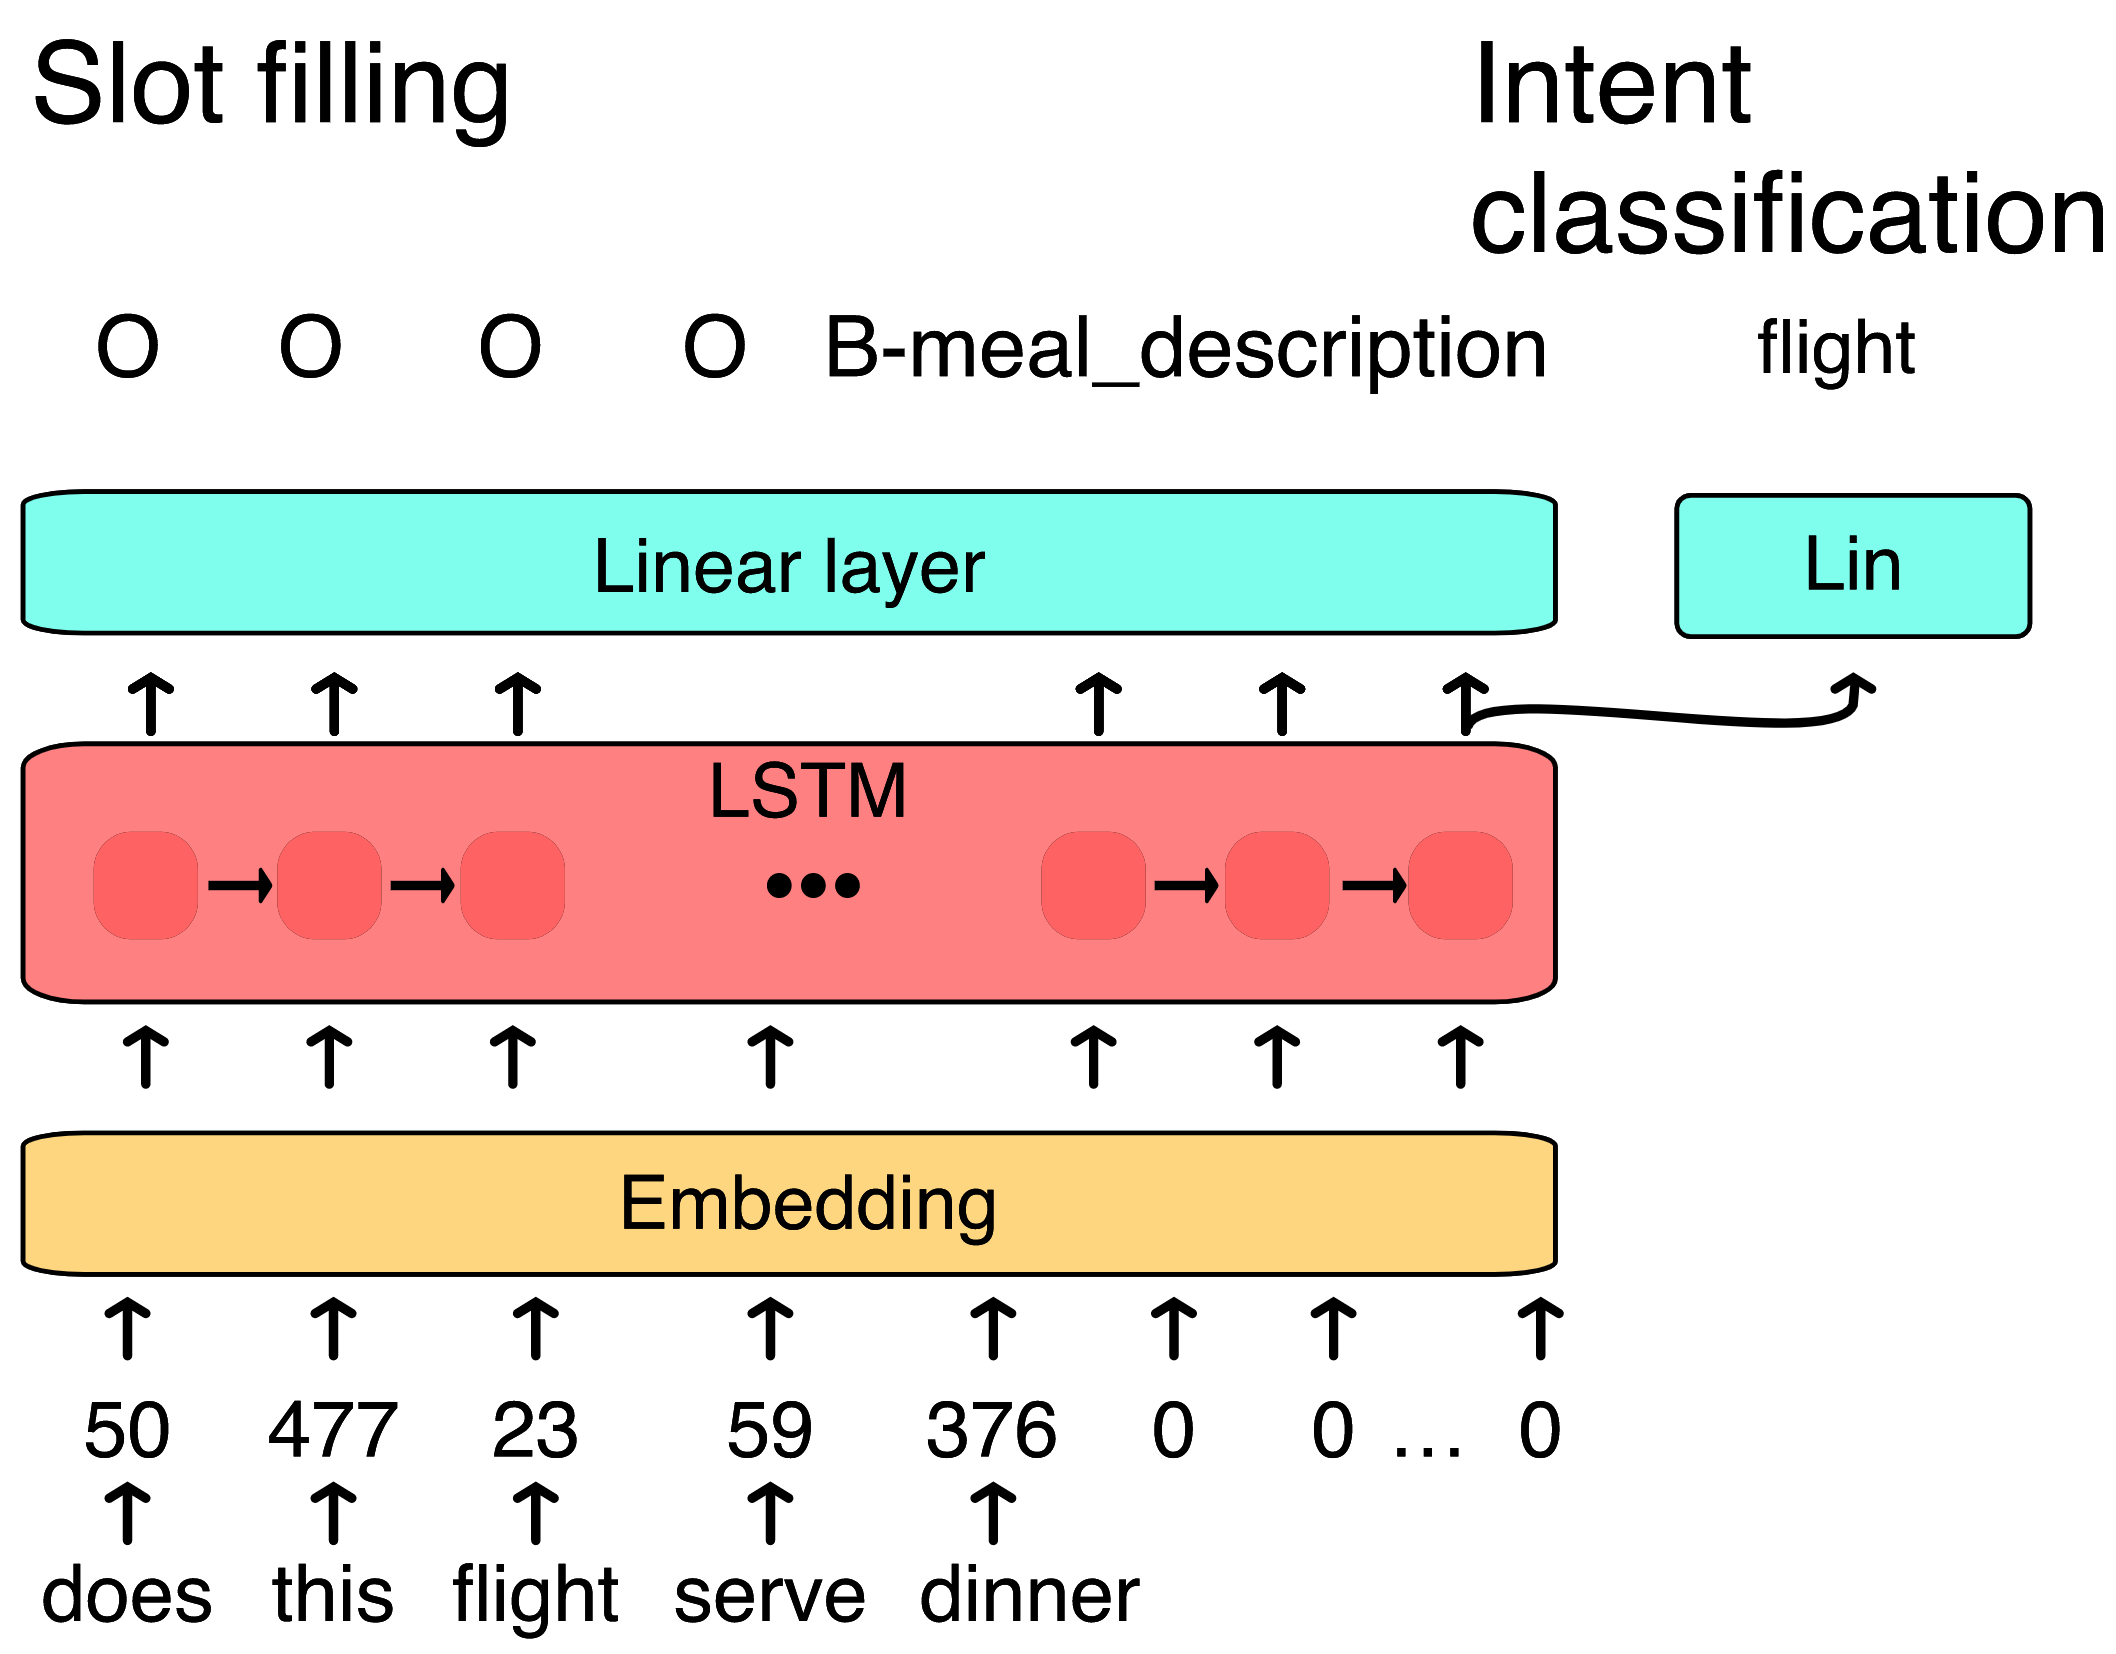
\includegraphics[width=0.8\linewidth]{../assets/images/baseline.png}
	\caption{baseline}
	\label{fig:Baseline}
\end{figure}
\begin{itemize}
	\item embedding layer
	\item LSTM with 1 layer
	\item output layers for slot filling and intent classification
\end{itemize}

\subsection{BiLSTM}
\begin{figure}[h!]
	\centering
	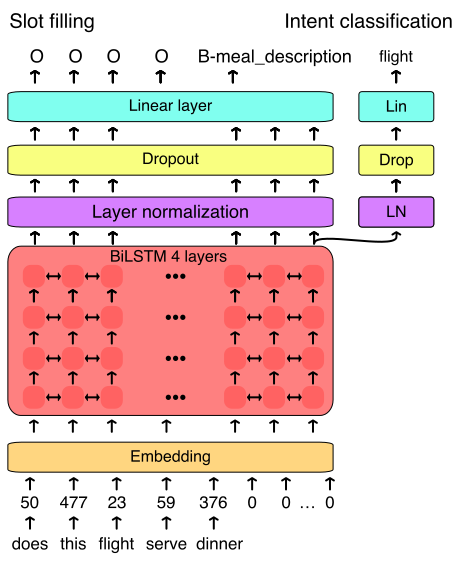
\includegraphics[width=0.8\linewidth]{../assets/images/BiLSTM}
	\caption{BiLSTM based}
	\label{fig:bilstm}
\end{figure}

This model is based on a bidirectional Long Short Term Memory network. The architecture is show in Fig \ref{fig:bilstm}

More specifically it consists of:
\begin{itemize}
	\item embedding layer
	\item bidirectional LSTM with 4 layers
	\item layer normalization
	\item dropout layer
	\item output layers for slot filling and intent classification
\end{itemize}

The model is composed by a BiLSTM as backbone, followed by two heads, one for slot filling and one for intent classification. Slot filling considers the whole encoded sentence by utilizing the hidden outputs from the last layer of the BiLSTM backbone. Intent classification only considers the last hidden state of the last layer to make the prediction.

\subsection{BERT}
\begin{figure}[h!]
	\centering
	\includegraphics[width=0.8\linewidth]{../assets/images/BERT}
	\caption{BERT based}
	\label{fig:bert}
\end{figure}
The second model proposed uses a similar architecture, but it replaces the embedding and BiLSTM with a BERT model as backbone. This was pre-trained from Huggingface, specifically \emph{bert-base-uncased}, which was trained using book-corpus and wikipedia datasets.  Due to lack of computational resources, the model was tested only once. Larger versions of BERT were not tried for similar reasons.

Because BERT is pre-trained on a different corpus, with a different task, it also expects a specific word to id encoding.

BertTokenizer is able parse the input sequence according to BERT needs, adding '[CLS]' and '[SEP]', two special tokens required by BERT. However the tokenizer also splits some tokens in base word and suffix. This creates an inconsistency with the number of slots. Therefore only the base word is considered and suffixes are ignored. Similarly '[CLS]' and '[SEP]' are removed in the slot filling. \\

%\centerline{how many people fit on a 72s airplane}
%\centerline{[CLS] how many people fit on a 72 \#\#s airplane [SEP]} 


%The results are shown in Table \ref{tab:tokenizer}

\begin{table}[h!]
	\centering
		\begin{adjustbox}{max width=0.5\textwidth}
				\begin{tabular}{l|l}
					\hline
						utterance & how many people fit on a 72s airplane\\
						BERT tokenization & [CLS] how many people fit on a 72 \#\#s airplane [SEP]\\
						\hline
				\end{tabular}
			\end{adjustbox}
		\vspace*{2mm}
		\caption{Example of tokenization differences}
		\label{tab:tokenizer}
\end{table}


The architecture is shown in Fig \ref{fig:bert} and it consists of:
\begin{itemize}
	\item BERT backbone
	\item layer normalization
	\item dropout
	%\item fully connected layers for slot filling and intent classification
	\item output layers for slot filling and intent classification
\end{itemize}

Intent classification takes as input the pooler\_output of the BERT backbone, which can be considered as the encoded token '[CLS]'.

Different learning rates for the classification layers and the backbone were used, specifically $e^{-4}$ and $e^{-5}$ respectively. This is to ensure that the model is able to learn the correct mapping for the classification layers and at the same time not lose the information stored in the pretrained backbone. 


Both simple architectures are complemented by a few considerations in order to improve performances.

\begin{itemize}
	\item early stopping
	\item random loss weighting
	\item focal loss
\end{itemize}

\subsection{Early stopping}

Early stopping is used to avoid overfitting. If both losses on slot filling and intent classification increase while training, the training is halted. Losses for early stopping are computed on the dev set. A hyperparameter for patience is set to 5 for both, which allows the model to increase the losses on the dev set up to 5 times before terminating.

%In figure \ref{fig::losses} is shown the effectiveness of early stopping.

%\begin{figure}
%	\centering
%	\begin{subfigure}[b]{width=0.4\linewidth}
%		\includegraphics[width=0.4\linewidth]{../BERT}
%		\caption{BiLSTM joint loss}
%		\label{fig:bilstm_loss}
%	
%	\end{subfigure}
%\hfill
%	\begin{subfigure}[b]{width=0.4\linewidth}
%		\includegraphics[width=0.4\linewidth]{../BERT}
%		\caption{BERT joint loss}
%		\label{fig:bert_loss}
%	\end{subfigure}
%	\label{fig:losses}
%\end{figure}

\subsection{Randomized loss weighting}

In multi task problems some tasks may converge earlier than others. Therefore weighting appropriately the losses for each task is not trivial and if done correctly it can improve performances. In \emph{A Closer Look at Loss Weighting in Multi-Task Learning} \cite{lin2022a}, the authors propose to chose weights of the losses randomly at each iteration. This simple strategy allows them to achieve results similar to more complex state of the art multi task loss weighting techniques. 

I use a very similar approach but with one key difference. I discovered that for both ATIS and SNIPS both models perform slightly better if among the two random weights, the larger is assigned to the task with higher loss. This is probably due to the fact that placing the larger weight to the task with higher loss increases the focus on that specific tasks. If one of the two tasks converges earlier, the loss will be lower and the smaller weight is assigned to the loss, as there is no need to learn more on that task. 

\subsection{Focal loss}
Finally, both models use a specific loss function. Instead of cross entropy, focal loss is used. It tackles the specific need for a loss that is better suited for classification on uneven datasets, with some labels that are easier or harder. It can be considered as a properly weighted cross-entropy loss, with highest loss to hard examples.

\begin{equation}
 FL = -\alpha(1-P_t)^\gamma log(P_t)
\end{equation}
with $\alpha$ and $\gamma$ two hyperparameters that regulate the weights placed on the labels.  

Optimizer used for both are Adam. Batch sizes are 128 for training set, 64 for validation and test set. 

%\begin{itemize}
%    \item \textit{your network/ algorithm (do not spend too much text in explaining already existing models, focus on your solution),}
%    \item \textit{the pipeline if used any, including  tokenizer, featurizer, extractor, etc.}
%    \item \textit{Your baseline and the experiments you have tried}
%\end{itemize}
% 

\section{Evaluation}

The main metrics used for evaluation are F1 score for slot filling and accuracy for intent classification. This is in line with the state of the art metrics on both ATIS and SNIPS for joint slot filling intent classification.

The final table here is shown in Tab \ref{tab:final_table}

Both models are far from the state of the art, but are a slight improvement over the baseline.

Confusion matrixes are reported in figures \ref{fig:cm_intent} and \ref{fig:cm_slot}
The colors are row normalized to prevent very frequent labels to dominate all the rest. 
Blank lines are where the models did not make any prediction for that specific label.

\begin{table*}[h!]
	\centering
	\begin{adjustbox}{max width=\textwidth}
		\begin{tabular}{l|ccc}
			Intent & & & \\
			Classification & & & \\
			& ATIS & balanced ATIS & SNIPS \\
			\cmidrule{1-4}
			Baseline &  \includegraphics[width=0.3\textwidth]{"../assets/images/confusion matrixes/CM_baseline_intent_ATIS_labeless"} & \includegraphics[width=0.3\textwidth]{"../assets/images/confusion matrixes/CM_baseline_intent_remix_ATIS_labeless"} &\includegraphics[width=0.3\textwidth]{"../assets/images/confusion matrixes/CM_baseline_intent_SNIPS_labeless"} \\
			\cmidrule{1-4}
			BiLSTM &  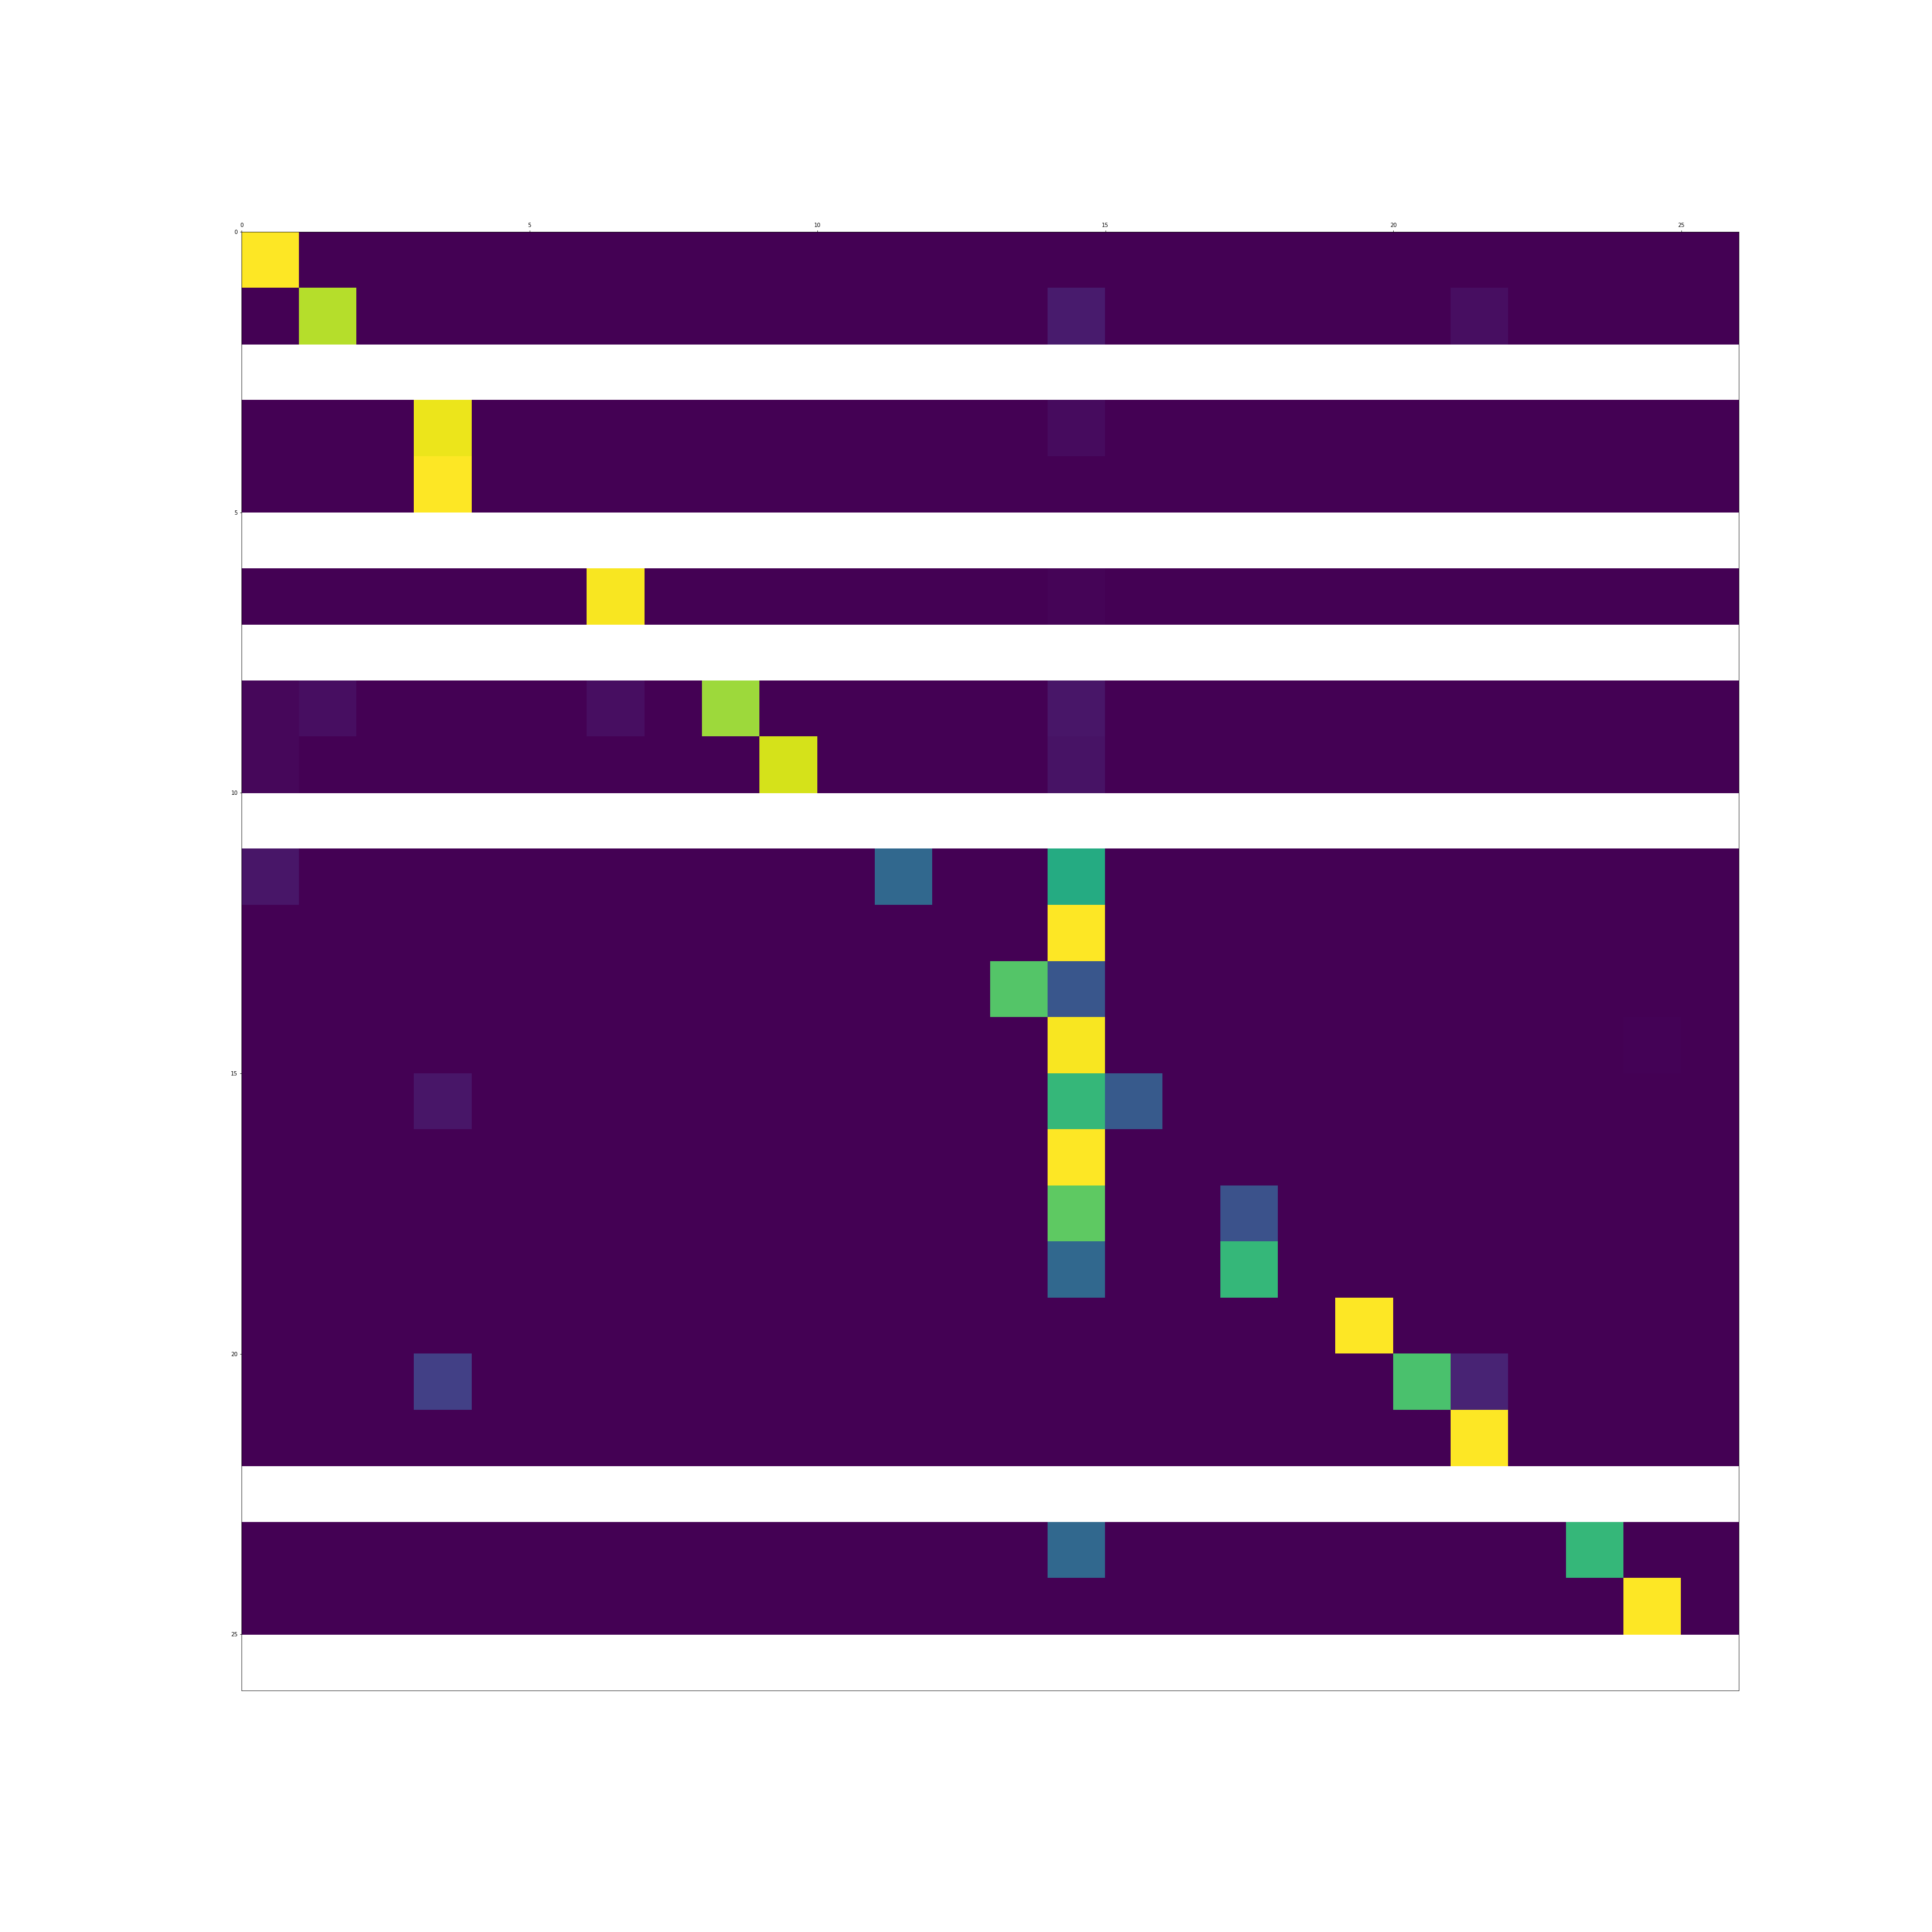
\includegraphics[width=0.3\textwidth]{"../assets/images/confusion matrixes/CM_BiLSTM_intent_ATIS_labeless.png"} & \includegraphics[width=0.3\textwidth]{"../assets/images/confusion matrixes/CM_BiLSTM_slot_remix_ATIS_labeless"}
			&\includegraphics[width=0.3\textwidth]{"../assets/images/confusion matrixes/CM_BiLSTM_intent_SNIPS_labeless"} \\
			\cmidrule{1-4}
			BERT &  \includegraphics[width=0.3\textwidth]{"../assets/images/confusion matrixes/CM_BERT_intent_ATIS_labeless"} &2 \includegraphics[width=0.3\textwidth]{"../assets/images/confusion matrixes/CM_BERT_intent_remix_ATIS_labeless"} &\includegraphics[width=0.3\textwidth]{"../assets/images/confusion matrixes/CM_BERT_intent_SNIPS_labeless"} \\
			%	Baseline &  \raisebox{-\totalheight}{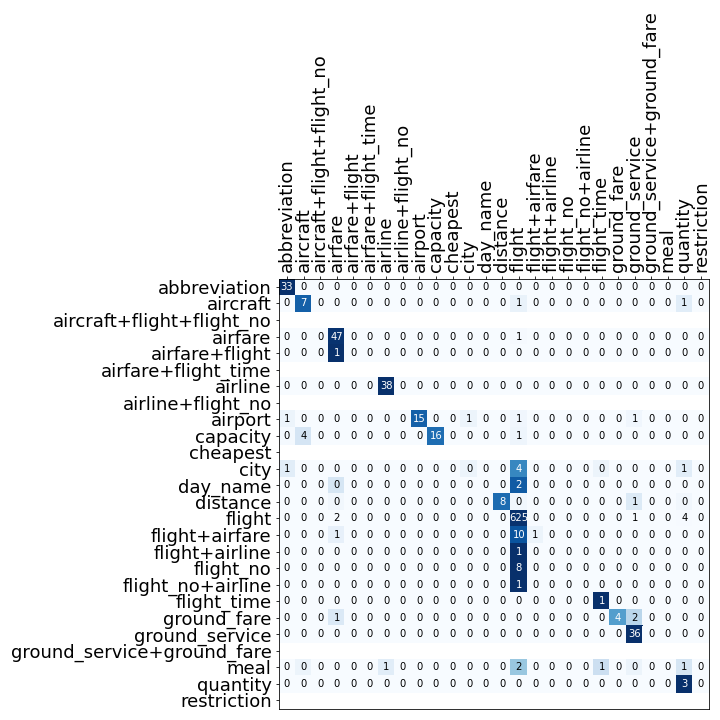
\includegraphics[width=0.3\textwidth, height=60mm]{../assets/images/CM_baseline_intent_ATIS}} & \raisebox{-\totalheight}{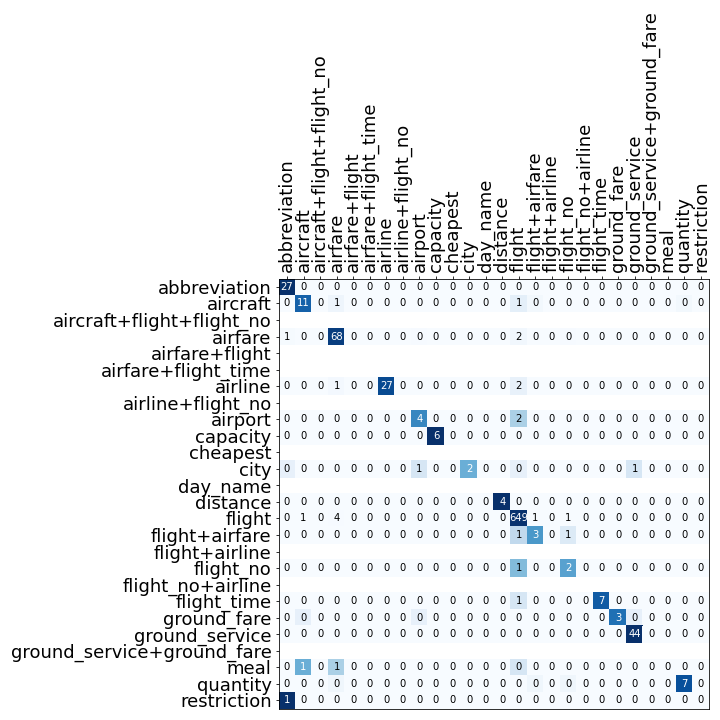
\includegraphics[width=0.3\textwidth, height=60mm]{../assets/images/CM_baseline_intent_remix_ATIS}} & \raisebox{-\totalheight}{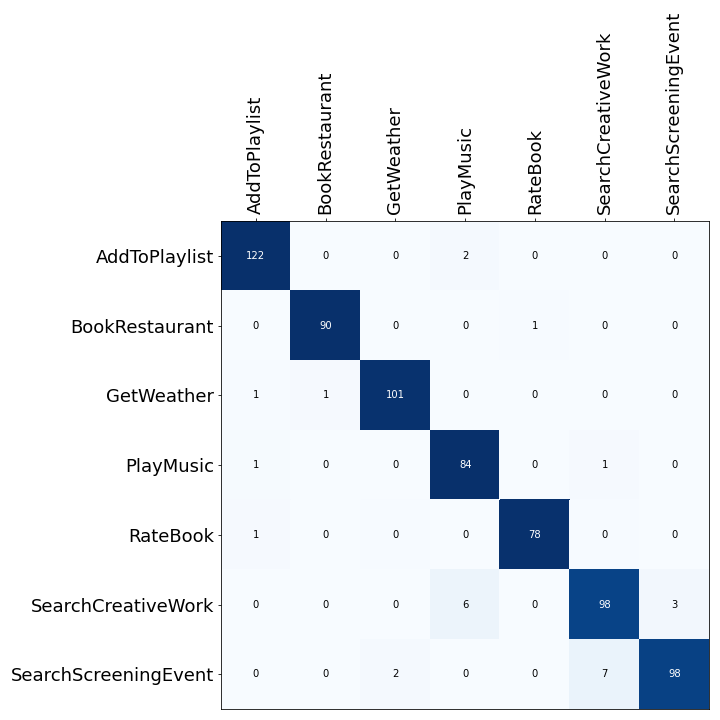
\includegraphics[width=0.3\textwidth, height=60mm]{../assets/images/CM_baseline_intent_SNIPS}}\\
		\end{tabular}
	\end{adjustbox}
\caption{Confusion matrixes for intent classification}
\label{fig:cm_intent}
\end{table*}

\begin{table*}[h!]
	\centering
	\begin{adjustbox}{max width=\textwidth}
		\begin{tabular}{l|ccc}
			Slot & & & \\
			Filling & & & \\
			& ATIS & balanced ATIS & SNIPS \\
			\cmidrule{1-4}
			Baseline &  \includegraphics[width=0.3\textwidth]{"../assets/images/confusion matrixes/CM_baseline_slot_ATIS_labeless"} & \includegraphics[width=0.3\textwidth]{"../assets/images/confusion matrixes/CM_baseline_slot_remix_ATIS_labeless"} &\includegraphics[width=0.3\textwidth]{"../assets/images/confusion matrixes/CM_baseline_slot_SNIPS_labeless"} \\
			\cmidrule{1-4}
			BiLSTM &  \includegraphics[width=0.3\textwidth]{"../assets/images/confusion matrixes/CM_BiLSTM_slot_ATIS_labeless"} & \includegraphics[width=0.3\textwidth]{"../assets/images/confusion matrixes/CM_BiLSTM_slot_remix_ATIS_labeless"} &\includegraphics[width=0.3\textwidth]{"../assets/images/confusion matrixes/CM_BiLSTM_slot_SNIPS_labeless"} \\
			\cmidrule{1-4}
			BERT &  \includegraphics[width=0.3\textwidth]{"../assets/images/confusion matrixes/CM_BERT_slot_ATIS_labeless"} & \includegraphics[width=0.3\textwidth]{"../assets/images/confusion matrixes/CM_BERT_slot_remix_ATIS_labeless"} &\includegraphics[width=0.3\textwidth]{"../assets/images/confusion matrixes/CM_BERT_slot_SNIPS_labeless"} \\
			%	Baseline &  \raisebox{-\totalheight}{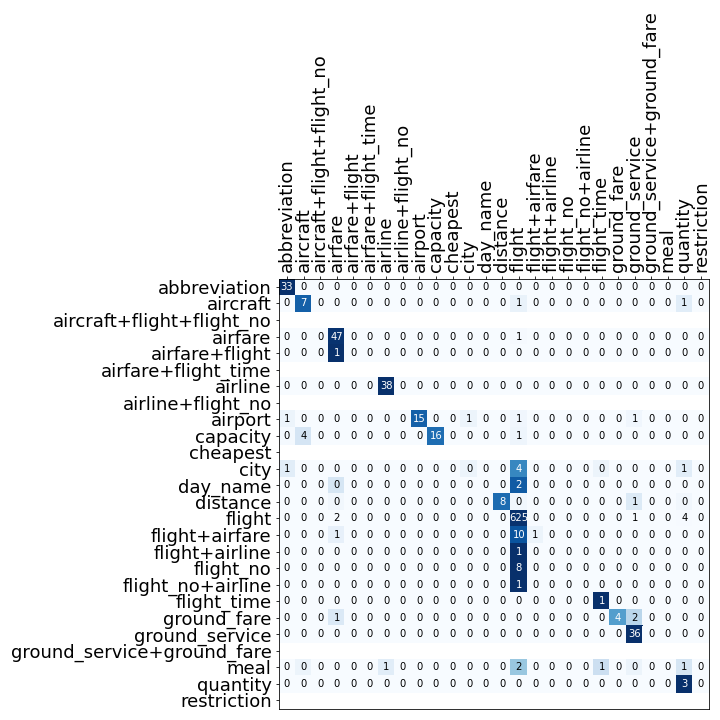
\includegraphics[width=0.3\textwidth, height=60mm]{../assets/images/CM_baseline_intent_ATIS}} & \raisebox{-\totalheight}{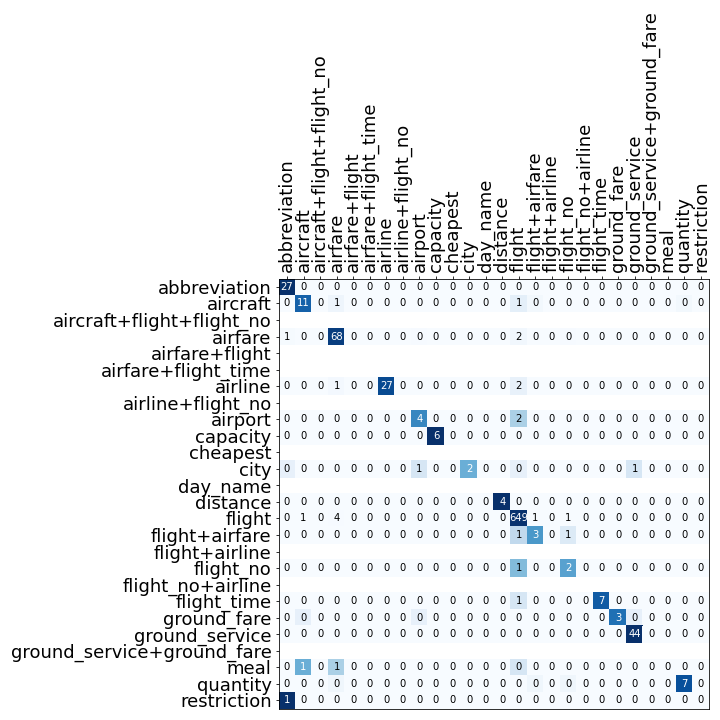
\includegraphics[width=0.3\textwidth, height=60mm]{../assets/images/CM_baseline_intent_remix_ATIS}} & \raisebox{-\totalheight}{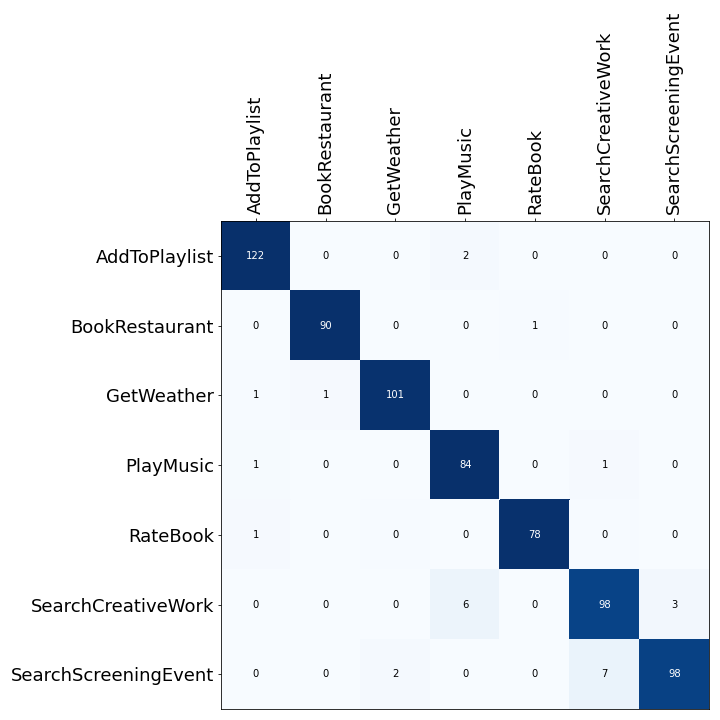
\includegraphics[width=0.3\textwidth, height=60mm]{../assets/images/CM_baseline_intent_SNIPS}}\\
		\end{tabular}
	\end{adjustbox}

\caption{Confusion matrixes for slot filling}
\label{fig:cm_slot}
\end{table*}

It is possible to see that for slot filling in ATIS, balanced ATIS and SNIPS, there is a vertical line on the label corresponding to 'O'. This is because 'O' is the most frequent label and therefore all models have a tendency to overpredict this label. Hard examples, that occur with few instances are also likely to be predicted 'O'. 

A similar consideration can be made for the label 'flight' in intent classification in ATIS. Intent classification on SNIPS does not show the same issue. 

In theory, balanced ATIS is an easier dataset to train, as it is more evenly distributed than ATIS. Although there are significant improvements on F1 score and accuracy for slot filling and intent classification, these advantages do not directly translate to a better confusion matrix. Because most of the blank lines correspond to labels that are not present in the train or dev sets, it would be expected that with a better partitioning, the number of blank lines would diminish. However this does not happen. Probably the reason lays in the very limited number of examples with those labels. 
It is also possible to notice that both in slot filling and intent classification, the models are less inclined to predict 'O' and 'flights' on balanced ATIS than default ATIS.

Although SNIPS is arguably a better dataset than ATIS, being larger, evenly distributed, with fewer labels and a bigger vocabulary, all models perform better on ATIS rather than SNIPS for intent classification and significantly worse on slot filling. The better performances for intent classification can be easily explained by the limited (7) number of labels. The worse results on slot filling may be caused by the scope of the tasks. 
On one hand, it is true that on ATIS there are more slot label, with fewer examples, but on the other hard all labels are under the wider scope of airport related requests. On SNIPS the requests cover a wider spectrum. This and the limited vocabulary on ATIS, probably lead to more examples for each token on ATIS than on SNIPS.


BERT performs much better than BiLSTM. Because this models it is based on a fine tuning of a pretrained model, this should solve the issue of having a small and biased dataset, fact that is corroborated by the data. 

Looking at the t-distributed stochastic neighbour embeddings (TSNE) in Fig\ref{tab:embeddings} the features extracted by each model, before the classification layers, it is clear that BERT achieve a much higher class separation of the labels leading to better performances. 

\begin{table*}[h!]
	\centering
%	\begin{adjustbox}{max width=\textwidth}
	\resizebox{\textwidth}{!}{%
		\begin{tabular}{l|cc|cc}
			&ATIS & & SNIPS & \\
			& Slot Embeddings & Intent Embeddings & Slot Embeddings& Intent Embeddings \\
			\cmidrule{1-5}
			Baseline &  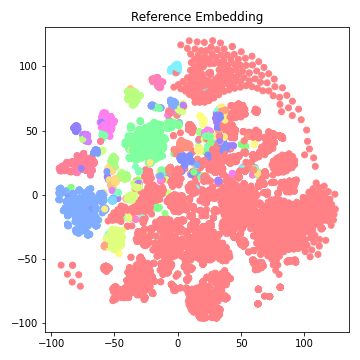
\includegraphics[width=0.2\textwidth]{"../assets/images/embeddings/baseline_slots_embeddings_ATIS_single.png"} &
			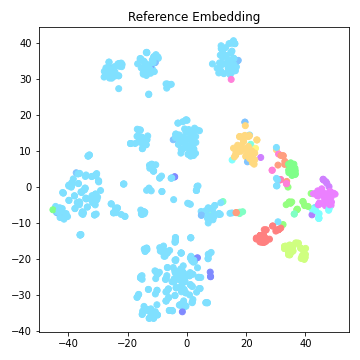
\includegraphics[width=0.2\textwidth]{"../assets/images/embeddings/baseline_intent_embeddings_ATIS_single.png"} &
			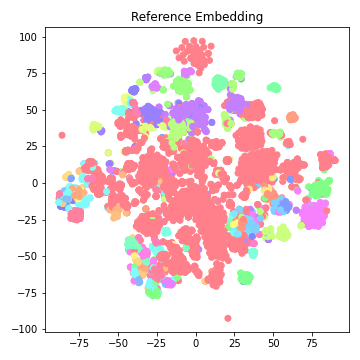
\includegraphics[width=0.2\textwidth]{"../assets/images/embeddings/baseline_slot_embeddings_SNIPS_single.png"} &
			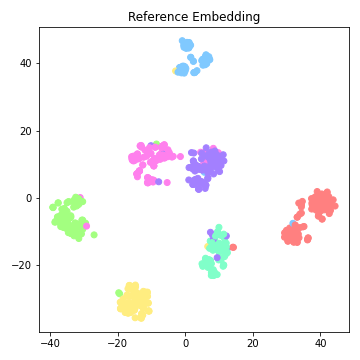
\includegraphics[width=0.2\textwidth]{"../assets/images/embeddings/baseline_intent_embeddings_SNIPS_single.png"} \\
			\cmidrule{1-5}
			BiLSTM &  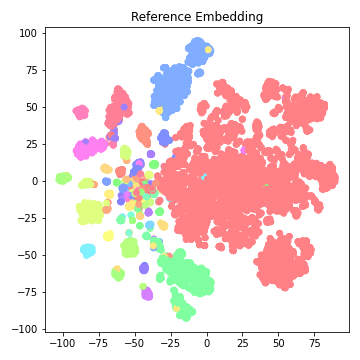
\includegraphics[width=0.2\textwidth]{"../assets/images/embeddings/BiLSTM_slot_embeddings_ATIS_single.png"} &
			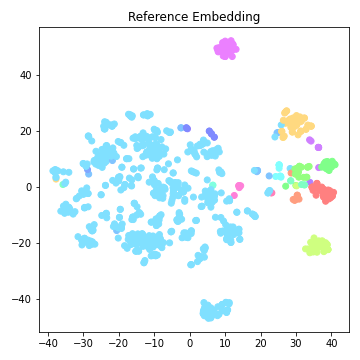
\includegraphics[width=0.2\textwidth]{"../assets/images/embeddings/BiLSTM_intent_embeddings_ATIS_single.png"} &
			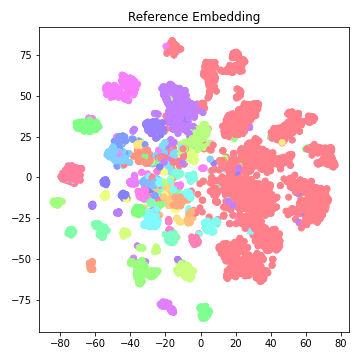
\includegraphics[width=0.2\textwidth]{"../assets/images/embeddings/BiLSTM_slot_embeddings_SNIPS_single.png"} &
			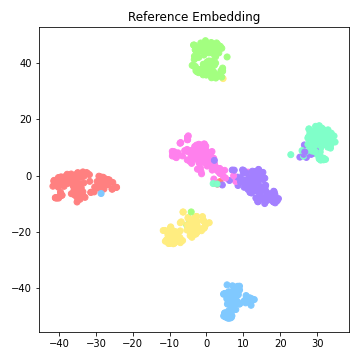
\includegraphics[width=0.2\textwidth]{"../assets/images/embeddings/BiLSTM_intent_embeddings_SNIPS_single.png"} \\
			\cmidrule{1-5}
			BERT &  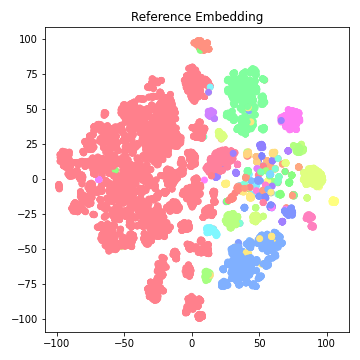
\includegraphics[width=0.2\textwidth]{"../assets/images/embeddings/BERT_slot_embeddings_ATIS_single.png"} &
			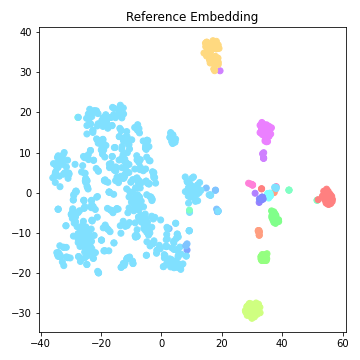
\includegraphics[width=0.2\textwidth]{"../assets/images/embeddings/BERT_intent_embeddings_ATIS_single.png"} &
			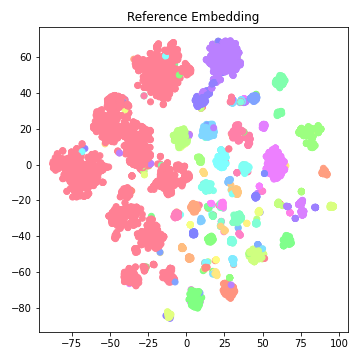
\includegraphics[width=0.2\textwidth]{"../assets/images/embeddings/BERT_slot_embeddings_SNIPS_single.png"} &
			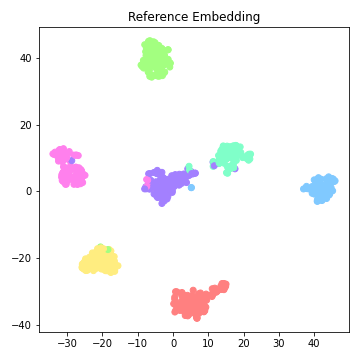
\includegraphics[width=0.2\textwidth]{"../assets/images/embeddings/BERT_intent_embeddings_SNIPS_single.png"} \\
			\cmidrule{1-5}
		\end{tabular}
%	\end{adjustbox}
	}
	
	\caption{TSNE of the features for each model. Notice that the clusters are better separated on BERT than on the other two models. In particular on intent classification, the labels that correspond to \textcolor{Myviolet}{SearchCreativeWork} and \textcolor{Mypurple}{SearchScreeningEvent} are well separated }
	\label{tab:embeddings}
\end{table*}

In 'BERT for Joint Intent Classification and Slot Filling' \cite{https://doi.org/10.48550/arxiv.1902.10909} the authors use a similar architecture and are able to perform much better on slot filling., however they are able to achieve slightly more. 


\begin{table*}[h!]
	\centering
	\begin{adjustbox}{max width=\textwidth}
		\begin{tabular}{*{7}{l}}%%{|c|c|c|c|c|c|c|c|c|c|c|c|c|c|}
			%			\hline
			Slot filling & & &\\
			\hline
			Model: & ATIS & & ATIS balanced & & SNIPS &\\
					& Slot F1 & Intent Acc 	& Slot F1 & Intent Acc 	& Slot F1 & Intent Acc \\
			\hline
			baseline & 92.06\% & 93.34\%& 94.43\%& 96.71\%& 80.27\%& 96.05\% \\
			1° proposal BiLSTM & 94.59\%& 94.89\%& 97.52\%& 97.24\%& 87.06\% & 96.14\%\\
			2° proposal BERT& 95.50\%& 97.31\%& 98.36\%& 98.43\%& 94.23\%& 97.71\%\\
			Some state of the art & & & & & & \\
			Joint BERT \cite{https://doi.org/10.48550/arxiv.1902.10909} & 96.1\%& 97.5\%& - & - & 97.0\%& 98.6\%\\
			Bi-model with decoder\cite{wang-etal-2018-bi} & 98.99\% & 96.89\% & - & - & - & - \\
			Stack-Propagation (+BERT) \cite{qin-etal-2019-stack} & 96.1\% & 97.5\% & - & - & 97.0\% & 99.0\% \\
			\hline
		\end{tabular}
	\end{adjustbox}
		\caption{results}
	\label{tab:final_table}
\end{table*}

%\begin{itemize}
%    \item \textit{The metrics you used}
%    \item \textit{Results on evaluation that you performed}
%    \item \textit{Comparison and differences between you model and the baseline}
%    \item \textit{Correct interpretation of errors and analysis}
%\end{itemize}

Looking at the training losses on BiLSTM in Fig \ref{fig:losses} a final remark.
\begin{figure}[h!]
	\centering
%	\begin{subfigure}[b]{0.3\textwidth}
%		\centering
%		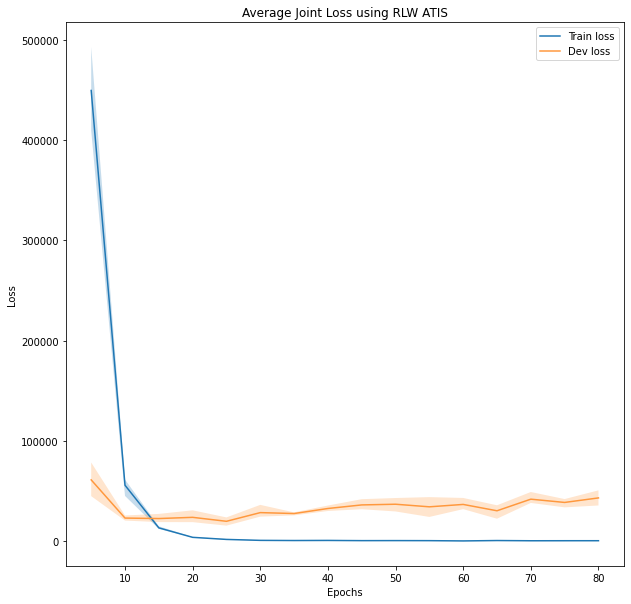
\includegraphics[width=\textwidth]{../assets/images/BiLSTM_joint_loss_ATIS.png}
%		%		\caption{This is a tiger.}
%	\end{subfigure}
	\begin{subfigure}[b]{0.22\textwidth}
		\centering
		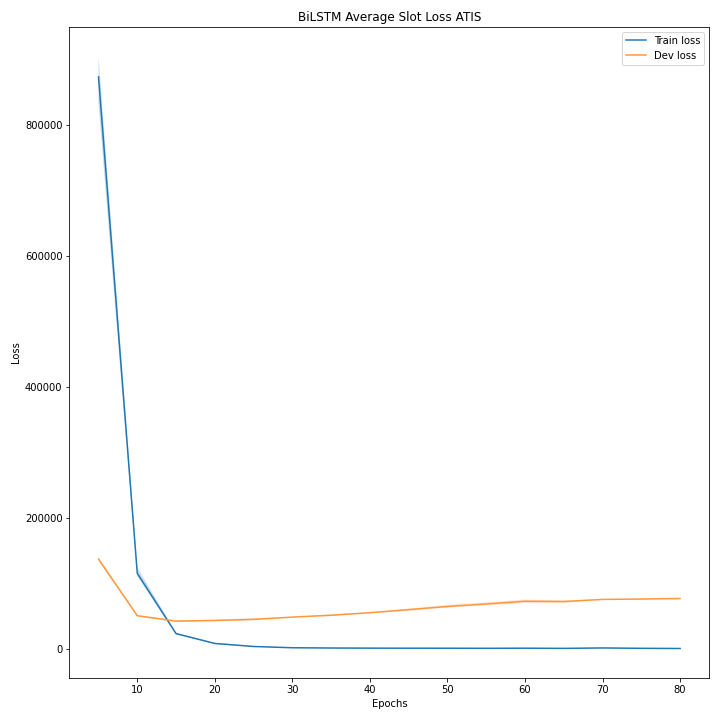
\includegraphics[width=\textwidth]{"../assets/images/losses/BiLSTM Average Slot Loss ATIS.png"}
				\caption{Slot Loss}
	\end{subfigure}	
	\hfill
	\begin{subfigure}[b]{0.22\textwidth}
		\centering
		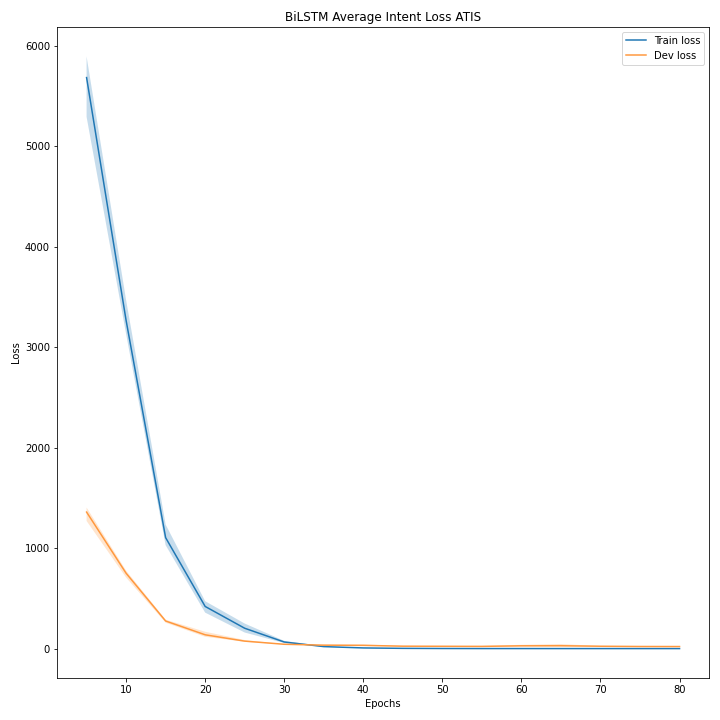
\includegraphics[width=\textwidth]{"../assets/images/losses/BiLSTM Average Intent Loss ATIS.png"}
				\caption{Intent Loss}
	\end{subfigure}
 \caption{Training losses of BiLSTM on ATIS. \textcolor{Myblue}{Train} and \textcolor{Myorange}{Dev} respectively}
 \label{fig:losses}
\end{figure}

Even using early stopping, the loss on slot filling does increase on the dev set. This is because the training stops only if both dev losses start to increase. I was unable to change the hyperparameters regulating early stopping to remove this issue without compromising results. If this issue is solved, it is very likely possible to increase the slot filling performances further.
\section{Conclusion}

I presented two models for the joint task of slot filling and intent classification. While neither are able to achieve results comparable to the state of the art, both are a marked improvement over a simple baseline model and BERT finetuning is not far from the state of the art

As future work, it would be possible to explore more complex architectures for both models presented. 

\bibliographystyle{IEEEtran}

\bibliography{mybib}
%
% \begin{thebibliography}{9}
%
% \bibitem[1]{Davis80-COP}
%   S.\ B.\ Davis and P.\ Mermelstein,
%   ``Comparison of parametric representation for monosyllabic word recognition in continuously spoken sentences,''
%   \textit{IEEE Transactions on Acoustics, Speech and Signal Processing}, vol.~28, no.~4, pp.~357--366, 1980.
% \bibitem[2]{Rabiner89-ATO}
%   L.\ R.\ Rabiner,
%   ``A tutorial on hidden Markov models and selected applications in speech recognition,''
%   \textit{Proceedings of the IEEE}, vol.~77, no.~2, pp.~257-286, 1989.
% \bibitem[3]{Hastie09-TEO}
%   T.\ Hastie, R.\ Tibshirani, and J.\ Friedman,
%   \textit{The Elements of Statistical Learning -- Data Mining, Inference, and Prediction}.
%   New York: Springer, 2009.
% \bibitem[4]{YourName17-XXX}
%   F.\ Lastname1, F.\ Lastname2, and F.\ Lastname3,
%   ``Title of your INTERSPEECH 2021 publication,''
%   in \textit{Interspeech 2021 -- 20\textsuperscript{th} Annual Conference of the International Speech Communication Association, September 15-19, Graz, Austria, Proceedings, Proceedings}, 2020, pp.~100--104.
% \end{thebibliography}

\end{document}
